\chapter{Before you start writing}

A dozen mistakes and bad choices can be made before even the first word of actual text is written.
In this chapter we talk about how to prevent this from happening.
Some of the points -- those about code quality and code management -- are not unique to writing {\LaTeX}.




\section{Use version control}

Use some kind of sensible version control\index{version control} for your code.
The author uses Git\index{Git} but has also heard good things about Mercurial\index{Mercurial}.
Sending code to yourself on Facebook\index{Facebook} is not a proper system of version control.





\section{Code quality}



\subsection{Make use of whitespace to organize the code}

The {\LaTeX} compiler almost never cares about unnecessary whitespace in your code.
Use generous amounts of whitespace to organize your code in a sensible way.
Don’t do the following:
\begin{showcode}{Code is too cramped}
\[\begin{pmatrix*}[r]a^2+b^2&a^2-b^2\\-a^2+b^2&-a^2-b^2\end{pmatrix*}\]
\end{showcode}
Instead do the following:
\begin{showcode}{Code is less cramped}
\[
  \begin{pmatrix*}[r]
     a^2 + b^2 &  a^2 - b^2 \\
    -a^2 + b^2 & -a^2 - b^2
  \end{pmatrix*}
\]
\end{showcode}
You can (and should) even do the following:
\begin{showcode}{Code isn’t cramped}
\[
  \begin{pmatrix*}[r]
    a^2 + b^2
    &
    a^2 - b^2
    \\
    - a^2 + b^2
    &
    - a^2 - b^2
  \end{pmatrix*}
\]
\end{showcode}
This last one is easiest to write and easiest to navigate.

Also put at least one space between any two symbols that do not belong together.
Don’t do the following:
\begin{showcode}{Unrelated symbols need to be separated}
$y=\sin(x)-e^x$
\end{showcode}
Instead do the following:
\begin{showcode}{Unrelated symbols are separated}
$y = \sin(x) - e^x$
\end{showcode}
One could (and probably should) go even further and do the following:
\begin{showcode}{Unrelated symbols are separated even better}
$y = \sin ( x ) - e^x$
\end{showcode}



\subsection{Write one sentence per line}

Related the previous point, write at most one sentence per line.
This has at least three advantages:
\begin{itemize}
  \item
    When an error\index{error} or warning\index{warning} occurs {\LaTeX} will (try to) tell you the line of source code in which the problem occurs.
    Having your source code split up over multiple lines makes it much easier to find the problem.
  \item
    Organizing the source code in lines will in most cases make the tools provided by your version control\index{version control} system more efficient to use.
  \item
    By writing one sentence per line you will more easily spot sentences which are overly long.
\end{itemize}



\subsection{Properly indent your source code}

Writing {\LaTeX} means writing source code.
Make sure that your source code is properly indented\index{indentation}.



\subsection{Use \inlinecodetitle{\%} for problematic line~breaks}

Sometimes a sensible line break in your source code can lead to unwanted effects in the resulting output.
Consider the following example:
\begin{showlatex}*{Wrong spacing before a footnote}
Here is some text.
\footnote{Here is a footnote for this text.}
\end{showlatex}
Note the unwanted space\index{before a footnote} between the period and the superscript of the footnote\index{footnote}.
This unwanted space comes from the line break that occurs between them in the source code.
By ending the first line with \inlinecode{\%}\massindex{\%}[\inlinecode] we can \enquote{comment out} this line break.
We hence do the following:
\begin{showlatex}*{Right spacing before a footnote}
Here is some text.%
\footnote{Here is a footnote for this text.}
\end{showlatex}





\section{The compilation process}



\subsection{Use \texorpdfstring{\LuaLaTeX}{LuaLaTeX} or \texorpdfstring{\XeLaTeX}{XeLaTeX}}

Use {\LuaLaTeX}\index{LuaLaTeX@{\LuaLaTeX}} or {\XeLaTeX}\index{XeLaTeX@{\XeLaTeX}} for native Unicode\index{Unicode} support (i.e.\ without including any kind of additional packages).
The author recommends {\LuaLaTeX} because the \packname{microtype}\massindex{microtype}[\packname] package his only a limited functionality under {\XeLaTeX}.



\subsection{Don’t ignore warnings}

There are two ways in which {\LaTeX} will tell you that something went wrong:
Errors\index{error} and warnings\index{warning}.

The occurrence of an error means that {\LaTeX} was unable the process the source code and gave up at some point in the process.
In the case of a warning {\LaTeX} again wasn’t able to process the source code, but decided to produce some output nevertheless.
Hence the only difference between an error and a warning is how {\LaTeX} decided to proceed with it.
But there is no intrinsic difference between the two of them.

It is typically hard to ignore errors, as no output file will be generated.
But warnings also shouldn’t be ignored:
While the occurrence of an error means that you get no output at all, the occurrence of a warning means that you’re getting a faulty output.

% TODO: Too many warnings make future problems worse.





\section{Splitting up a project into multiple files}
\index{including files!zzzz@\igobble |see{file inclusion}}

Any slightly larger project should be split up into multiple files.



\subsection{The commands~\comtitle{usepackage}, \comtitle{include}, \comtitle{input}}

There are (at least) three useful ways to include another file into your project: \comname{usepackage}\massindex[file inclusion]{usepackage}[\comname], \comname{include}\massindex[file inclusion]{include}[\comname] and \comname{input}\massindex[file inclusion]{input}[\comname].
\begin{itemize}[leftmargin=*]
  \item
    Most of the preamble information -- including of packages, configuration of styles, configuration of the look and feels of the document -- should be put into one or multiple \filename{sty}-files.
    These file(s) can then be included into the document by using \comname{usepackage}\massindex[file inclusion]{usepackage}[\comname].
  \item
    The commands~\comname{include} and~\comname{input} insert the text of the specified documents at the position where they are used, but have slight differences:
    \begin{itemize}[label = \textopenbullet, leftmargin=*]
      \item
        The command~\comname{include}\massindex[file inclusion]{include}[\comname] ensures that the specified content starts on a new page, and also that the following content begins on a new page.
        The command~\comname{input}\massindex[file inclusion]{input}[\comname] simply inserts the specified content at the given position without any such additional formatting.
      \item
        The command~\comname{include} cannot be nested:
        The specified file is not allowed to include the command~\comname{include} again.
    \end{itemize}
\end{itemize}

One should use the command~\comname{include} for chapters and the command~\comname{input} for any smaller level of text organization.
One should in particular break the main text into smaller units until each of them can be put into its own file of sensible length.

Suppose for example that your text consists of three chapters, each of which consists of two sections.
Then you should have at least ten files:
\begin{itemize}
  \item
    A master file \filename{main.tex}.
    This file includes all other files in some way, and this is the file which needs to be compiled.
  \item
    A file \filename{mystyle.sty} in which packages are included and options are set.
  \item
    Three files like \filename{chapter1.tex}, \filename{chapter2.tex} and \filename{chapter3.tex} for the chapters.
  \item
    Six files for the sections, say \filename{section1.tex} up to \filename{section6.tex}.
\end{itemize}
These files should include each other as shown in \cref{file inclusion structure}.
\begin{figure}[tb]
  \begin{center}
    % the following diagram uses the "trees" library
    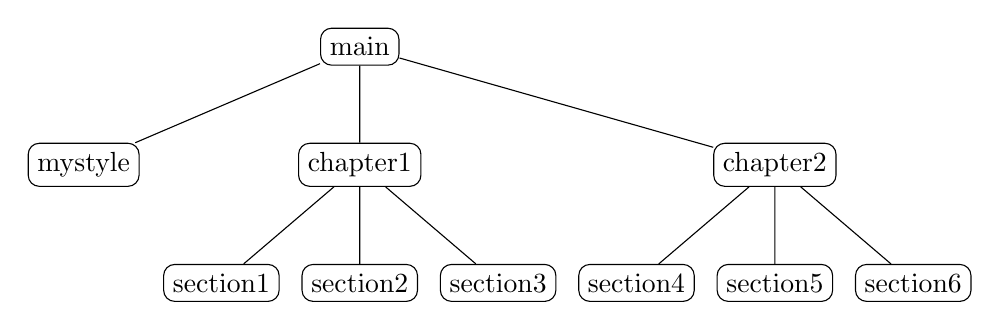
\begin{tikzpicture}[
      every node/.style = {shape=rectangle, rounded corners, draw, align=center},
      level 1/.style = {sibling distance = 15em},
      level 2/.style = {sibling distance = 5em}
      ]
      \node {\filename{main}}
        child { node [right=3em] {\filename{mystyle}} }
        child { node {\filename{chapter1}}
          child { node {\filename{section1}} }
          child { node {\filename{section2}} }
          child { node {\filename{section3}} }
        }
        child { node {\filename{chapter2}}
          child { node {\filename{section4}} }
          child { node {\filename{section5}} }
          child { node {\filename{section6}} }
        };
    \end{tikzpicture}
  \end{center}
  \caption{Splitting up a project into files.}
  \label{file inclusion structure}
\end{figure}
We suppose for simplicity that all ten files are contained in the same directory.
The master file \filename{main.tex} should look roughly as follows:
%
\begin{showcode}{Layout of \filename{main.tex}}
\documentclass[a4paper, 10pt]{scrreprt}

\usepackage{mystyle}

\title{A Report}
\author{John Doe}

\begin{document}

\maketitle

\include{chapter1}
\include{chapter2}

\end{document}
\end{showcode}
%
The file \filename{mystyle.sty} may look as follows:
%
\begin{showcode}{Layout of \filename{mystyle.sty}}
%%%%% PACKAGES

% general mathematics
\usepackage{mathtools}
\usepackage{amssymb}

% commutative diagrams
\usepackage{tikz-cd}

%%%%% NEW COMMANDS

% new operators
\DeclareMathOperator{\End}{End}
\DeclareMathOperator{\Hom}{Hom}
\end{showcode}
%
The file \filename{chapter1.tex} should look roughly as follows:
%
\begin{showcode}{Layout of \filename{chapter1.tex}}
\chapter{Name of the first chapter}

Some introduction to this chapter before the first section appears.

\input{section1}
\input{section2}
\end{showcode}
%
The file \filename{section1.tex} should look roughly as follows:
%
\begin{showcode}{Layout of \filename{section1.tex}}
\section{Name of the first section}

Text of the first section.
\end{showcode}



\subsection{Use \comtitle{includeonly}}

As a document grows so does the time that is needed to compile it.
It is therefore often desirable to compile only certain parts of the document.
One naive solution to this problem is to simply not include the currently unwanted parts, e.g.\ by commenting out the corresponding lines of~\comname{include} and~\comname{input}.
This approach has the problem that references to the now-excluded parts of the document will not compile properly.
This problem can be fixed by using the command~\comname{inludeonly}\massindex[file inclusion]{includeonly}[\comname].

Suppose that your main document, say \filename{main.tex}, included two other files, say \filename{chapter1.tex} and \filename{chapter2.tex}, via the command \comname{include}.
Hence the file~\filename{main.tex} should look roughly as follows:
\begin{showcode}{Basic example of \filename{main.tex}}
\documentclass[a4paper, 10pt]{scrreprt}

\begin{document}

\include{chapter1}
\include{chapter2}

\end{document}
\end{showcode}
By putting~\inlinecode{{\tbs}includeonly\{chapter1\}} in the preamble we tell {\LaTeX} to only compile this specific chapter.
\begin{showcode}{Using the command~\comname{includeonly}}
\documentclass[a4paper, 10pt]{scrreprt}

\includeonly{chapter1}
\begin{document}

\include{chapter1}
\include{chapter2}

\end{document}
\end{showcode}
If in the above situation chapter~1 contains some references to chapter~2 then these references will still compile correctly, even though only chapter~1 is compiled.

The command~\comname{includeonly} has two quirks, which follow from the way {\LaTeX} handles referencing:

When {\LaTeX} compiles the file~\filename{main.tex} an auxiliary file~\filename{main.aux} is created.
This file contains various information about the compiled document.
It does in particular contain a list of all labels found in \filename{main.tex} during the compilation process.
The next compilation process can then access these information to properly properly typeset all references that refer to these labels.

A feature of the command~\comname{include} (which the command~\comname{input} does not have) is that such an auxiliary file is also generated for the included file.
So in the above example the files~\filename{chapter1.aux} and \filename{chapter2.aux} will be created.
These files will in particular contain lists of all the labels found in~\filename{chapter1.tex} and \filename{chapter2.tex}.
This allows {\LaTeX} to access the labels in \filename{chapter2.tex} even though only \filename{chapter1.tex} is compiled.

The auxiliary file~\filename{chapter2.aux} remains unchanged because {\LaTeX} does not go trough the file~\filename{chapter2.tex} as long as the code~\inlinecode{{\tbs}includeonly\{chapter1\}} is used.
This leads to the two quirks mentioned above:
\begin{itemize}
  \item
    Before inserting the code \inlinecode{{\tbs}includeonly\{chapter1\}} one needs to compile the whole document, including \filename{chapter2.tex}, a least once.
    This needs to be done so that {\LaTeX} can properly create the auxiliary file~\filename{chapter2.aux}.
  \item
    Changes made to the file~\filename{chapter2.tex} will not be noticed by {\LaTeX} while the code~\inlinecode{{\tbs}includeonly\{chapter1\}} is present.
    This means in particular that {\LaTeX} won’t notice any new labels that are added in this file.
    In this case one need to stop excluding \filename{chapter1.tex} for at least on compilation process to ensure that the auxiliary file~\filename{chapter2.aux} is refreshed.
\end{itemize}

The command~\comname{includeonly} actually accepts as its argument a list of files to be included:
\begin{showcode}{Syntax of \comname{includeonly}}
  \includeonly{file_1, ..., file_n}
\end{showcode}





\section{Choosing the document class}



\subsection{Use the KOMA-Script classes}

Instead of the standard classes\index{standard classes} \optname{article}\massindex[standard classes, document class!classes]{article}[\optname], \optname{report}\massindex[standard classes, document class!classes]{report}[\optname] or \optname{book}\massindex[standard classes, document class!classes]{book}[\optname] the the more modern KOMA-Script classes \optname{scrartcl}\massindex[KOMA-Script classes, document class!classes]{scrartcl}[\optname], \optname{scrreprt}\massindex[KOMA-Script classes, document class!classes]{scrreprt}[\optname] and \optname{scrbook}\massindex[KOMA-Script classes, document class!classes]{scrbook}[\optname] should be used.
They provide more functionalities then the standard classes and a more unified interface.

The KOMA-Script classes make slightly different design choices than the standard classes:
\begin{itemize}
  \item
    The KOMA-Script classes have a different chapter title layout than the standard classes.
    The standard look can be regained by setting the option~\optname{chapterprefix}\massindex[KOMA-Script classes, document class!options]{chapterprefix}[\optname] to~\optname{true}:
    \begin{showcode}{Using the option~\optname{chapterprefix}}
\documentclass[10pt, a4paper, chapterprefix = true]{scrbook}
    \end{showcode}
  \item
    The default font of the KOMA-Script classes for headings and description~labels is a bold sans-serif font.
    It can be changed to the standard serif font with help of the command~\comname{setkomafont}\massindex[KOMA-Script classes, fonts]{addtokomafont}[\comname].
    \begin{showcode}{Changing KOMA fonts}
\addtokomafont{disposition}{\rmfamily}
\addtokomafont{descriptionlabel}{\rmfamily}
    \end{showcode}
%     One can also make the heading be in small capitals instead of boldface by replacing~\comname{bfseries}\massindex[fonts]{bfseries}[\comname] by~\comname{scshape}\massindex[fonts]{scshape}[\comname].
  One can also use the undocumented option~\optname{egregdoesnotlikesansseriftitles}\massindex[KOMA-Script classes, document class!options]{egreg\-does\-not\-like\-sans\-serif\-titles}[\optname].
  \begin{showcode}{Using the option~\optname{egregdoesnotlikesansseriftitles}}
\documentclass[10pt, a4paper, egregdoesnotlikesansseriftitles]{scrbook}
  \end{showcode}
\end{itemize}



\subsection{Deciding on a document class}
\index{document class}

The three standard classes to consider for a mathematical project are~\optname{scrartcl}\massindex[KOMA-Script classes, document class!classes]{scrartcl}[\optname],~\optname{scrreprt}\massindex[KOMA-Script classes, document class!classes]{scrreprt}[\optname] and~\optname{scrbook}\optionindex{scrbook}{scrbook}\massindex[KOMA-Script classes, document class!classes]{scrbook}[\optname].
These three classes differ in what functionalities they provide and what they standard settings are.

The class~\optname{scrartcl} is the most basic one.
It provides the standard sectioning commands~\comname{section}\massindex[sectioning]{section}[\comname],~\comname{subsection}\massindex[sectioning]{subsection}[\comname] and~\comname{subsubsection}\massindex[sectioning]{subsubsection}[\comname].
An abstract can be set with the~\envname{abstract}\massindex{abstract}[\envname] environment and by giving~\comname{documentclass} the option~\inlinecode{abstract~=~on}\massindex[document class!options]{abstract}[\envname]:
\begin{showcode}{Using the environment~\envname{abstract}}
\documentclass[10pt, a4paper, abstract = on]{scrartcl}

\begin{document}

\begin{abstract}
  Our results are cool and our proofs have no details.
\end{abstract}

\end{document}
\end{showcode}

The class~\optname{scrreprt} extends the previous class:
It provides the additional sectioning command~\comname{chapter}\massindex[sectioning]{chapter}[\comname] that precedes~\comname{section}.
The title is now printed its own page, although this can by setting the option~\optname{titlepage}\massindex[KOMA-Script classes, document class!options]{titlepage}[\optname] to~\optname{false}:
\begin{showcode}{Using the option~\optname{titlepage}}
\documentclass[10pt, a4paper, titlepage = false]{scrreprt}
\end{showcode}
It also provides the sectioning command~\comname{abstract} after which all chapters will be counted towards the appendix.
The~\envname{abstract} environment is still available in the same way as before.
(But the abstract is printed only on the second page, after the title page.)

The class~\optname{scrbook} provides the additional sectioning command~\comname{part}\massindex[sectioning]{part}[\comname] that precedes~\comname{chapter}.
This class also provides the (very useful) additional sectioning commands~\comname{frontmatter}\massindex[sectioning]{frontmatter}[\comname],~\comname{mainmatter}\massindex[sectioning]{mainmatter}[\comname] and~\comname{backmatter}\massindex[sectioning]{backmatter}[\comname].
The~\envname{abstract} environment isn’t available anymore.
This class distinguish between left and right pages, i.e.\ even and odd pages.
This can be disabled by using the option~\optname{oneside}\massindex[KOMA-Script classes, document class!options]{oneside}[\optname]:
\begin{showcode}{Using the option~\optname{oneside}}
\documentclass[10pt, a4paper, oneside]{scrbook}
\end{showcode}
By default chapters will begin on the right side.
This can be disabled with the option~\optname{openany}\massindex[KOMA-Script classes, document class!options]{openany}[\optname]:
\begin{showcode}{Using the option~\optname{openany}}
\documentclass[10pt, a4paper, openany]{scrbook}
\end{showcode}
When the option~\optname{oneside} is used then chapters can start on both the left pages and the right pages.
So option~\optname{openany} is then not needed.

In practice one should use the class~\optname{scrartcl} if only sections and subsections are used, and otherwise the class~\optname{scrbook}.
Instead of~\optname{scrreprt} one should directly use~\optname{scrbook}:
The additional commands~\comname{frontmatter},~\comname{mainmatter} and~\comname{backmatter} that~\optname{scrbook} provides are extremely useful (see \cref{using frontmatter}), and the visual difference between~\optname{scrreprt} and~\optname{scrbook} (which is their main difference) can easily be adjusted by passing the option~\optname{openany}\massindex[KOMA-Script classes, document class!options]{openany}[\optname] to~\comname{documentclass}:
\begin{showcode}{Using the option~\optname{openany}}
\documentclass[10pt, a4paper, openany]{scrbook}
\end{showcode}





\section{Use \comtitle{frontmatter} and its friends}
\label{using frontmatter}

The class~\optname{scrbook} provides the commands~\comname{frontmatter}\massindex[sectioning]{frontmatter}[\comname],~\comname{mainmatter}\massindex[sectioning]{mainmatter}[\comname] and\comname{backmatter}\massindex[sectioning]{backmatter}[\comname].
Together with the sectioning command~\comname{appendix}\massindex[sectioning]{appendix}[\comname] these can be used to separate the document into four parts:
The front part, the main part, the appendix and the back part.
These parts behave slightly differently:
\begin{itemize}
  \item
    The front part uses lower case roman numerals\index{roman numerals}\index{numerals!roman} for page numbers.
    In the generated \pagename{pdf}-file these pages will again be numbered with roman numerals (this will be important for the main part).
    Chapters in this part of the document will not be numbered, but will appear in the table of contents.
    
    This part of the document should include the title page\index{title page}, preface\index{preface}, table of content\index{table of contents} and introduction\index{introduction}.
    Basically everything that occurs before the first chapter.
  \item
    The main part uses Arabic numerals\index{Arabic numerals}\index{numerals!Arabic} for page numbers and the page number is reset when the main part starts.
    The first page of the main part is therefore numbered~\enquote{1}.
    In the generated \filename{pdf}-file this first page will also be numbered as such.
    This means that going to page~15 of the \filename{pdf}-file will indeed give page~15 of the document.
    The chapters in this part of the document are numbered and appear in the table of contents.
    
    This part of the document does contain the vast amount of the document.
    It contains all the chapters excluding the ones belonging into the appendix.
  \item
    The appendix part continues the numbering of the main part.
    It both resets the chapter number and changes its style to upper case letters.
    The first chapter in this part will hence be numbered~\enquote{A}.
    If the option~\inlinecode{chapterprefix~=~true} is set then the word~\enquote{Chapter} at the beginning of a new~\comname{chapter} will be replaced by~\enquote{Appendix}.
    
    This part of the document should contain all appendices.
  \item
    The back part continues the numbering of the appendix (and thus the numbering of the main part).
    The chapters appearing in this part of the document are again unnumbered, and no~\enquote{Chapter} is printed at the beginning of a new~\comname{chapter} is printed.
    
    This part of the document should contain the bibliography and the index.
    An entry for the bibliography\index{bibliography} can be added to the table of contents by setting the option~\optname{bibliography}\massindex[KOMA-Script classes, document class!options, bibliography]{bibliography}[\optname] to~\optname{totoc}\massindex[KOMA-Script classes]{totoc}[\optname].
\end{itemize}

The document layout with~\optname{scrbook} should therefore look roughly as follows:

\begin{showcode}[label = {layout for scrbook}]{General document layout with~\optname{scrbook}}
\documentclass[a4paper, 10pt,bibliography=totocnumbered]{scrbook}

% preamble

\begin{document}

\frontmatter
\maketitle
% dedication
% preface
\tableofcontents
% introduction

\mainmatter
% most of the document

\appendix
% the appendices

\backmatter
\printbibliography
% index
\end{document}
\end{showcode}





\section{Be consistent}

One of the most important aspects of both mathematical writing and the use of mathematical notation is consistency\index{consistency}.
If you’re making crappy choices then at least do them consistently, in the same way.
Consider the following example:
% 
% \begin{tcblisting}{title = {Bad}}
% % in the preamble:
% \newcommand{\glie}{\mathfrak{g}}
% % in the main text:
% The algebra $U(\glie)$ is commutative if and only if the original Lie algebra $\glie$ is abelian.
% But $\operatorname{U}(\glie)$ is infinite dimensional whenever $\glie$ is nonzero, even if $\glie$ itself is finite dimensional as well.
% \end{tcblisting}
% Even if the reader doesn’t care if you use $U(\mathfrak{g})$ or $\operatorname{U}(\mathfrak{g})$ they will notice the inconsistent use of the two notations, and this will distract them from the actual content of the text.
% 
% We consider another example:
\begin{showlatex}{Inconsistency looks bad}
If $X$ and $Y$ are two objects in a category $\mathcal{C}$ then it may happen that the set $\operatorname{Hom}_{\mathcal{C}}(X,Y)$ is empty even though the set $Hom_{\mathcal{C}}(Y,X)$ is non-empty.
\end{showlatex}
The inconsistent use of~$Hom$ and~$\operatorname{Hom}$ makes the already bad~$Hom$ even worse.




